\documentclass[11pt,a4paper]{article}
\usepackage[T1]{fontenc}
\usepackage[utf8]{inputenc}
\usepackage[brazil]{babel}
\usepackage{lmodern}
\usepackage[margin=2.2cm]{geometry}
\usepackage{amsmath,amssymb}
\usepackage{graphicx}
\usepackage{booktabs}
\usepackage{array}
\usepackage{caption}
\usepackage{float}
\usepackage{xcolor}
\usepackage[hidelinks]{hyperref}
\captionsetup{font=small,labelfont=bf}
\renewcommand{\thetable}{R\arabic{table}}
\renewcommand{\thefigure}{R\arabic{figure}}
\newcommand{\Gam}{\Gamma}
\newcommand{\gradu}{-\mathrm{grad}\,u'_{\mathrm{FE}}}
\newcommand{\vopt}{\underline{\underline{K}}\cdot\underline{v}'_{\mathrm{opt}}}
\newcommand{\Gart}{\Gamma_{\mathrm{artigo}}}
\newcommand{\Gfe}{\Gamma_{\mathrm{FE}}}
\newcommand{\Hcrit}{H_{\mathrm{crit}}}
\definecolor{art}{RGB}{184,57,43}

\title{Talude sob rebaixamento com variabilidade espacial:\\ reprodução de Vargas Ceron et al.\ (2025) com o NeoPZ}
\author{Projects2/SlopeSeepageRandom --- relatório comparativo}
\date{\today}

\begin{document}
\maketitle

\begin{abstract}
Os exemplos de M.~Vargas Ceron, D.~L.~Cecílio, R.~V.~Linn e S.~Maghous, \emph{Stability Analysis of Slope Subjected to
Seepage Forces Considering Spatial Variability of Soil Properties} (IJNAMG 49, 2025, 2459--2491) foram recalculados
com o NeoPZ: elastoplasticidade Mohr-Coulomb incremental, fluxo de Darcy por elementos finitos e campos aleatórios de
Karhunen-Loève. O artigo usa a análise limite cinemática com mecanismos log-espirais. Este relatório compara as
análises determinísticas (Figs.~5, 8 e 9, Tabelas~5 e 6 e exemplos de Cho do artigo) e o Monte Carlo de todos os casos
das Tabelas~3 a 6 e da seção~5.3 do artigo, com 12.850 amostras (390 a 500 por caso), e
estima o tempo para chegar ao número de amostras do artigo. Tabelas e figuras deste relatório são numeradas R1, R2,
\ldots; as do artigo são citadas como ``Tabela~3 do artigo'', ``Fig.~8 do artigo'' etc.
\end{abstract}

\tableofcontents

\section{Resumo dos resultados}
\begin{itemize}
\item \textbf{Reprodutibilidade.} Nas amostras em comum entre duas máquinas (o container de desenvolvimento e a máquina do autor, 631 amostras) e entre os dois pacotes de resultados recebidos (2800 amostras), os resultados são idênticos em todos os dígitos gravados ($\Gam$ e médias dos campos; modo de ruptura nas 431 amostras do container que o registram); cada amostra depende só de (semente, índice da amostra, campo).
\item \textbf{Exemplos secos (Cho).} No talude $c$-$\varphi$ o FE converge para logo abaixo do limite superior do artigo, como esperado: $\Gam = 1{,}764$ (nível 4) contra 1,777 e FS $= 1{,}202$ contra 1,203 (artigo) e 1,204 (Cho). No coesivo ainda decresce: $\Gam = 1{,}317$ e FS $= 1{,}324$ no nível 3 (cerca de 0,6\,\% por nível, $-$2{,}7\,\% em relação a 1,354; Cho: 1,356).
\item \textbf{Caso de referência com percolação.} O último fator convergido no FE refinado é $\Gam = 1{,}398$ e o colapso ocorre em 1{,}407--1{,}412, isto é, $+$4{,}7\,\% a $+$5{,}7\,\% acima do $\Gam = 1{,}336$ do artigo, que é um limite superior. Com $\gamma_w = 9{,}81$ (inferido da Fig.~8 do artigo), a diferença não vem da malha mecânica nem do tamanho do domínio para $\alpha = 1$; $\gamma_w = 10$ reduziria $\Gam$ em 1{,}9\,\%, o que não fecha a diferença. O restante é atribuído, por exclusão, às forças de percolação. Com anisotropia soma-se o efeito do domínio truncado (laterais impermeáveis a 10\,m do talude): com 50\,m de crista, pé e base, a diferença de $\alpha = 3$ e $5$ cai para $+$5{,}7\,\% e $+$5{,}1\,\% (nível 3, $\beta = 45^\circ$; $\alpha = 1$ no mesmo nível e domínio: $+$6{,}4\,\%).
\item \textbf{Fig.~8 do artigo.} Com os solos trocados em relação à Tabela~1 do artigo (seção~\ref{sec:obs}), o FE reproduz as curvas ${\gradu}$ com diferença de no máximo 3{,}8\,\% em três das quatro curvas (nível 3). Na quarta ($\varphi = 32^\circ$, $\beta = 35^\circ$) o FE fica 16 a 26\,\% abaixo para $h_w/H \ge 0{,}2$ (nível 3) e continua diminuindo com o refinamento; em $h_w/H = 0{,}1$ fica $+$14\,\% e sem rebaixamento não converge com a malha. Como as outras três curvas concordam, o limite superior do artigo provavelmente não é justo nesse caso ($\varphi$ próximo de $\beta$, mecanismo raso junto à face).
\item \textbf{Monte Carlo, média e desvio.} Nos 26 casos com percolação (Tabelas~3 a 6 do artigo) a média de $\Gam$ do FE é em média 8{,}8\,\% maior que a do artigo, o mesmo viés do problema médio na malha do Monte Carlo. Reescalada amostra a amostra por $\Gart/\Gfe$ do problema médio, coincide com a do artigo (diferença média $-$0{,}3\,\%, máxima 3{,}9\,\%); o desvio padrão reescalado é em média 12\,\% maior.
\item \textbf{Monte Carlo, probabilidade de falha.} O Pf do artigo está no intervalo de confiança de 95\,\% do FE em 16 dos 28 casos. Nos casos com percolação ele fica entre o Pf do FE (menor, pelo viés da média) e o Pf reescalado (maior, pelo desvio maior) em 24 dos 26 casos (exceções: $h_w/H = 0{,}5$ e $h_w/H = 0{,}6$, em que o Pf do FE já é maior que o do artigo), e dentro de pelo menos um dos dois intervalos de confiança em 18 dos 26. As tendências principais das Tabelas~3 a 6 do artigo se repetem (Pf com CoV$(c)$, CoV$(\varphi)$, $s$, $\alpha$ e $h_w/H$; $\sigma$ e CoV com $s$; $\mu$ com $\alpha$ e $h_w/H$); variações pequenas ($\mu$ com CoV$(\varphi)$ e com $s$, oscilações de $\sigma$ entre valores vizinhos de $s$) ficam dentro do ruído amostral.
\item \textbf{Cho.} Coesivo: $\mu = 1{,}232$, $\sigma = 0{,}199$ contra 1{,}279 e 0{,}201 da Fig.~17 do artigo; Pf $= 10{,}8\,\%$ contra 6,5\,\% (artigo) e 7,9\,\% (Cho). $c$-$\varphi$: a mediana coincide (1{,}669 contra 1{,}670); $\sigma = 1{,}129$ é dominado por uma amostra extrema ($\Gam = 17{,}4$; sem ela, $\sigma = 0{,}859$), contra 0{,}82--0{,}94 no artigo (Figs.~21 e 22); Pf $= 7{,}6\,\%$ contra 5,5\,\% e 6,37\,\%.
\item \textbf{Sensibilidade e modos de ruptura.} Correlações parciais de Spearman de 2ª ordem com médias no mecanismo: $c$ 0{,}88, $\varphi$ 0{,}55, $k_v$ $-$0{,}21 (artigo: 0,88, 0,51, $-$0,04); a correlação com $k_v$ é fraca nos dois, mais negativa no FE.
Cho coesivo: 100{,}0\,\% das rupturas abaixo do pé (artigo 92,7\,\%); Cho $c$-$\varphi$: 94{,}9\,\% pelo pé e 5{,}1\,\% acima (artigo 80,8\,\% e 19,2\,\%).
\item \textbf{Previsão.} Na máquina do autor (8 processos; 3{,}4--4{,}2\,s por amostra nos casos com percolação, 2{,}4\,s no Cho $c$-$\varphi$ e 37\,s no Cho coesivo) faltam 2{,}7\,h para $N = 1000$ por caso, 7{,}6\,h para $N = 2000$ e 8{,}1 dias para o número de amostras do artigo, 65\,\% disso no Cho coesivo.
\end{itemize}
\section{O que foi calculado}
\subsection{Formulação}
O artigo avalia a estabilidade pelo fator $\Gam$ (eq.~54 do artigo), multiplicador das cargas $\gamma'\,\underline{e}_y
- \mathrm{grad}\,u$ no colapso, obtido pela análise limite cinemática com mecanismos log-espirais rotacionais (limite
superior). As forças de percolação vêm de uma solução semianalítica em velocidade de filtração ($\vopt$) ou de
elementos finitos em poropressão (${\gradu}$). O $\Gam = 1{,}336$ do caso de referência (seção~6 e Tabelas~5 e 6 do
artigo) corresponde à curva ${\gradu}$: a Fig.~9 do artigo dá 1,31 em $\beta = 45^\circ$, $\alpha = 1$ para
${\gradu}$, contra 1,89 para $\vopt$ (a diferença de 1,7\,\% entre o valor digitalizado, 1,314, e 1,336 excede um
pouco a precisão de leitura, $\pm 0{,}01$).

O código (\texttt{Projects2/SlopeSeepageRandom} do NeoPZ) calcula o mesmo $\Gam$ como o multiplicador das mesmas
cargas no colapso de uma análise elastoplástica incremental: Mohr-Coulomb associado
(\texttt{TPZPlasticStepVoigt<TPZYCMohrCoulombPV2>}), quadriláteros de ordem 2, colapso definido pela não
convergência do Newton com bissecção do passo até 0,5\,\%. O excesso de poropressão $u$ é a solução de Darcy
estacionário (H1, ordem 2) com as condições de contorno da eq.~21 do artigo e laterais e base impermeáveis. Para a
plasticidade perfeita associada a carga de colapso é única: o FE em deslocamentos converge para ela de cima com o
refinamento, e o mecanismo log-espiral é um limite superior. A comparação direta é, portanto, com as curvas ${\gradu}$
do artigo, e um FE convergido abaixo do valor do artigo indica um limite superior pouco justo.

\subsection{Parâmetros numéricos}
\begin{itemize}
\item $\gamma_w = 9{,}81$\,kN/m$^3$. O artigo não informa $\gamma_w$; os valores da Fig.~8 do artigo sem
rebaixamento só são reproduzidos com 9,81 (com 10 a diferença é de 2,3 a 2,5\,\%).
\item Domínio: crista de 10\,m, pé de 10\,m e base 5\,m abaixo do pé ($25 \times 10$\,m no talude de referência, com
$H = 5$\,m e $\beta = 45^\circ$). Malha estruturada com $h = 1$\,m e refinamento adaptativo guiado pelo mecanismo de
colapso do problema médio. No Monte Carlo, dois níveis: 4914 equações no caso de referência, 18.014 no Cho coesivo
e 3194 no Cho $c$-$\varphi$ ($h = 2$\,m, $H = 10$\,m).
\item Campos aleatórios: KL de Galerkin (quadriláteros de 9 nós, $h_{\mathrm{KL}} = 1$\,m) com todos os modos da KL
discreta ($M$ = número de equações da malha KL: 871, 1081 e 1491); lognormais, covariância exponencial
$\exp(-|\Delta x|/L_x - |\Delta y|/L_y)$, $c$, $\varphi$ e $k_v$ independentes. O erro de discretização da variância
é $\varepsilon_M \approx 3{,}6\,\%$ para $(L_x, L_y) = (20, 2)$\,m (0,007 a 2,3\,\% nos casos da Tabela~4 do artigo),
compensado ponto a ponto. O artigo usa $M = 2000$ termos com erro abaixo de 6\,\%, sem compensação.
\item Monte Carlo direto, $P_f = P(\Gam < 1)$, intervalo de confiança de 95\,\% de Wilson. Colunas com~$^*$:
cada amostra multiplicada por $\Gart/\Gfe$ do problema médio na mesma malha e domínio, o que retira a diferença
determinística e deixa só o efeito da variabilidade.
\item Dados do artigo: tabelas e texto transcritos; Figs.~5, 8, 17, 21, 22 e 26 extraídas dos vetores do PDF e
Fig.~9 digitalizada da imagem, cada uma conferida por um segundo método (diferença máxima de 1,7\,\% nos pontos
lidos). Os momentos $\mu$ e $\sigma$ dos exemplos de Cho foram calculados dessas curvas e têm incerteza maior
(seção~4.1).
\end{itemize}

\section{Análises determinísticas}
\subsection{Convergência com a malha}\label{sec:conv}
A Tabela~\ref{tab:conv} mostra $\Gam$ e FS (redução de resistência) do problema médio para níveis crescentes de refinamento adaptativo.
\begin{table}[H]\centering\small\caption{Convergência com a malha (nível = número de refinamentos adaptativos; $h = 1$\,m, ou 2\,m no exemplo $c$-$\varphi$). $\Gam$ é o último fator de carga convergido.}\label{tab:conv}
\begin{tabular}{llrrrrrrr}\toprule exemplo & & nível 0 & 1 & 2 & 3 & 4 & 5 & artigo\\\midrule
Cho coesivo & $\Gam$ & 1{,}347 & 1{,}332 & 1{,}325 & 1{,}317 & 1{,}230 & --- & 1,354\\
 & FS & 1{,}353 & 1{,}341 & 1{,}332 & 1{,}324 & --- & --- & 1,354$^a$\\
Cho $c$-$\varphi$ ($H = 10$\,m) & $\Gam$ & 2{,}138 & 1{,}897 & 1{,}809 & 1{,}774 & 1{,}764 & --- & 1,777\\
 & FS & 1{,}272 & 1{,}232 & 1{,}208 & 1{,}204 & 1{,}202 & --- & 1,203$^b$\\
referência (Tab.~2 do artigo) & $\Gam$ & 1{,}649 & 1{,}537 & 1{,}453 & 1{,}425 & 1{,}398 & 1{,}398 & 1,336\\
 & FS & 1{,}312 & 1{,}258 & 1{,}222 & 1{,}208 & 1{,}131 & 1{,}204 & ---\\
\bottomrule\end{tabular}\\[2pt]{\footnotesize $^a$ $\Gam = F_s$ para $\varphi = 0$; Cho (2010), equilíbrio limite: 1,356. $^b$ Cho (2010): 1,204.}\end{table}
Nos exemplos secos o FE decresce com o refinamento e fica abaixo do limite superior do artigo (logo abaixo no $c$-$\varphi$; no coesivo ainda decresce cerca de 0,6\,\% por nível); para o $c$-$\varphi$, a solução log-espiral de Chen (1975), reimplementada aqui, dá $\Gam = 1{,}7770$ e $F_s = 1{,}203$ com $H = 10$\,m, os valores do artigo. No caso com percolação o último fator convergido é 1{,}398 nos níveis 4 e 5 e com $h = 0{,}5$\,m e 3 níveis, e o colapso ocorre em 1{,}407--1{,}412; a diferença em relação ao artigo é de $+$4{,}7\,\% a $+$5{,}7\,\%.
Variações do caso de referência (nível 3): $\gamma_w = 10$ dá $\Gam = 1{,}398$ (com 9,81: 1{,}425); o domínio de $105 \times 55$\,m dá 1{,}422. Nenhuma das duas fecha a diferença em relação ao artigo; o restante é atribuído, por exclusão, às forças de percolação (malha e domínio do FE hidráulico do artigo não são informados).
Nos níveis mais finos aparecem quedas isoladas fora da sequência: FS = 1{,}131 (referência, nível 4) e 1{,}172 ($h = 0{,}5$\,m, nível 3), e $\Gam = 1{,}230$ no Cho coesivo, nível 4 (20 cortes de passo; a execução foi interrompida antes do FS). As quedas de FS são colapsos prematuros do critério de não convergência do Newton em malhas muito finas; o valor do Cho coesivo no nível 4 não foi confirmado e não é usado. Com $h = 1$\,m, os níveis 2 e 3 usados nas comparações não apresentam o problema. Na seção~\ref{sec:f8} dois valores de nível 4 (9 e 10 cortes de passo) aparecem só como indicação da tendência; as conclusões usam o nível 3.
\subsection{Anisotropia e tamanho do domínio}\label{sec:dom}
\begin{table}[H]\centering\small\caption{$\Gam$ (nível 3, $\beta = 45^\circ$) para três domínios (crista/pé/base). Laterais e base impermeáveis.}\label{tab:dom}
\begin{tabular}{lrrrr}\toprule $\alpha$ & 10/10/5\,m & 25/25/15\,m & 50/50/50\,m & artigo\\\midrule
1 & 1{,}425 & --- & 1{,}422 & 1,336\\
3 & 1{,}847 & --- & 1{,}770 & 1,674\\
5 & 2{,}120 & 2{,}000 & 1{,}968 & 1,872\\
\bottomrule\end{tabular}\end{table}
Com $k_h > k_v$ as laterais impermeáveis próximas bloqueiam o fluxo horizontal e reduzem as forças de percolação; com o domínio grande a diferença em relação ao artigo volta ao patamar de $\alpha = 1$. O efeito do domínio foi verificado só em $\beta = 45^\circ$ e $\alpha \le 5$. No Monte Carlo ele é compensado pelas colunas reescaladas, que usam o $\Gam$ determinístico no mesmo domínio.
\subsection{Fig.~5 do artigo: funcional hidráulico}
\begin{figure}[H]\centering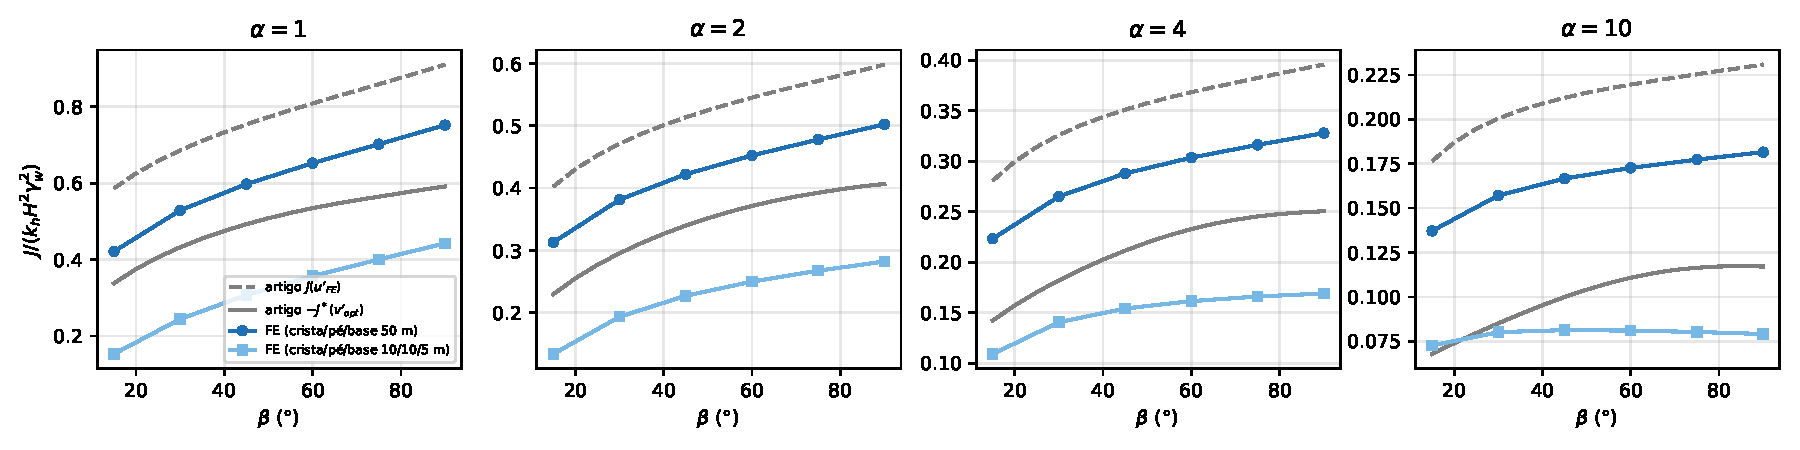
\includegraphics[width=\textwidth]{figuras/fig5_funcional}\caption{$J(u)/(k_h H^2\gamma_w^2)$ do FE em poropressão (malha convergida) para dois domínios (crista/pé/base 10/10/5\,m e 50/50/50\,m), com as estimativas do artigo $J(u'_{\mathrm{FE}})$ (tracejada) e $-J^*(\underline{v}'_{\mathrm{opt}})$ (contínua); só o domínio grande fica entre elas em todos os pontos.}\label{fig:f5}\end{figure}
O funcional depende do tamanho do domínio, que o artigo não informa para o FE. Com crista, pé e base de 50\,m (o $L_m = 10H$ do modelo semianalítico), o valor do FE fica entre as duas estimativas do artigo para todos os $\beta$ e $\alpha$, como exige a eq.~28 do artigo; com 10/10/5\,m ele fica abaixo da estimativa inferior em 23 dos 24 pontos (a exceção é $\alpha = 10$, $\beta = 15^\circ$).
\subsection{Fig.~8 do artigo: altura crítica com rebaixamento}\label{sec:f8}
Como o problema é autossemelhante, $\Hcrit = \Gam \cdot H$ com domínio e malha escalados com $H$ ($\gamma = 18$\,kN/m$^3$, $\alpha = 1$, 20\,m de crista e de pé, 10\,m de base). O solo A tem $c = 6$\,kPa e $\varphi = 32^\circ$; o B, $c = 11{,}7$\,kPa e $\varphi = 24{,}7^\circ$.
\begin{figure}[H]\centering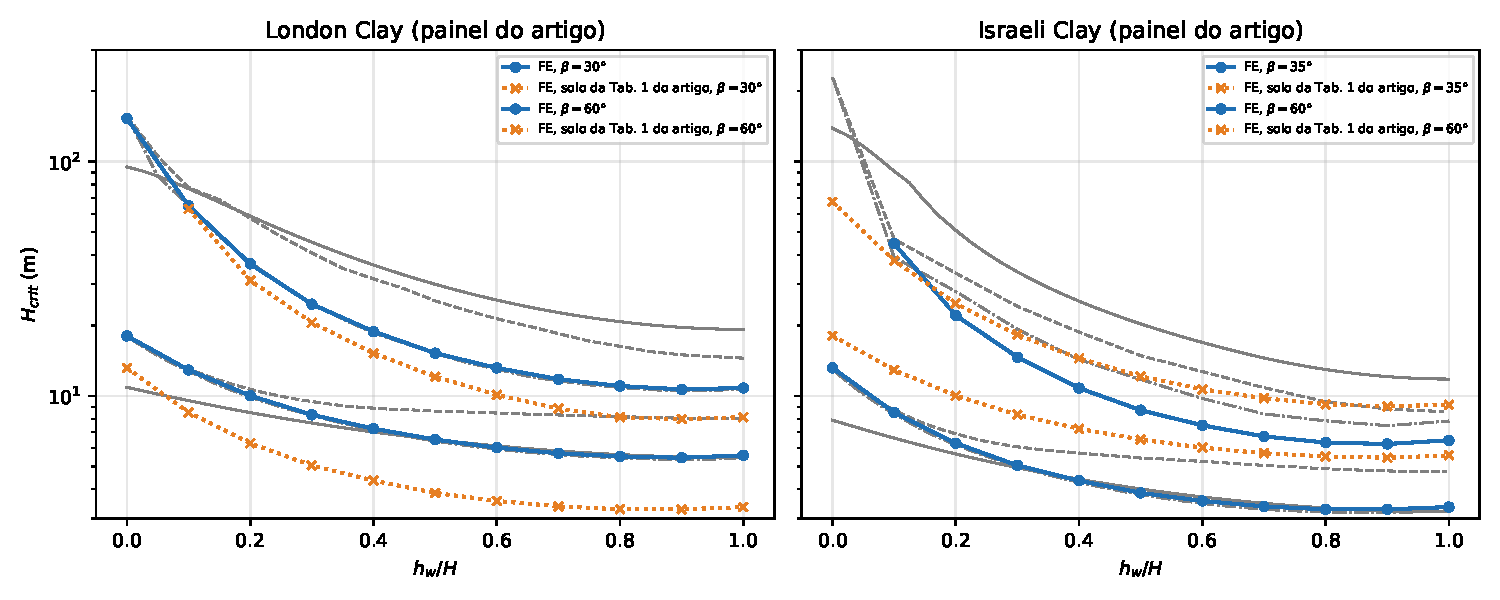
\includegraphics[width=\textwidth]{figuras/fig8_hcrit}\caption{Fig.~8 do artigo (cinza: contínua $r_p = 0{,}25$ de Wu et al.; tracejada $\vopt$; traço-ponto ${\gradu}$) e FE (azul: solo que reproduz o artigo em $h_w = 0$; laranja: solo da Tabela~1 do artigo para o rótulo do painel), nível 3.}\label{fig:f8}\end{figure}
\begin{table}[H]\centering\small\caption{$\Hcrit$ (m): FE (nível 3, que ainda diminui cerca de 1 a 3\,\% por nível de refinamento) contra a curva ${\gradu}$ do artigo. n.c.: sem convergência com a malha.}\label{tab:f8}
\begin{tabular}{llrrrrrrr}\toprule painel (solo) & $\beta$ & & \multicolumn{6}{c}{$h_w/H$}\\\cmidrule(l){4-9} & & & 0{,}0 & 0{,}2 & 0{,}4 & 0{,}6 & 0{,}8 & 1{,}0\\\midrule
London (B) & $30^\circ$ & FE & 153{,}2 & 36{,}7 & 18{,}9 & 13{,}2 & 11{,}0 & 10{,}8\\
 &  & artigo & 156{,}6 & 37{,}3 & 18{,}6 & 13{,}0 & 10{,}9 & 10{,}8\\
 &  & dif. & $-$2{,}1\,\% & $-$1{,}6\,\% & $+$1{,}2\,\% & $+$1{,}2\,\% & $+$1{,}4\,\% & $+$0{,}5\,\%\\
\addlinespace
London (B) & $60^\circ$ & FE & 18{,}1 & 10{,}0 & 7{,}3 & 6{,}0 & 5{,}5 & 5{,}6\\
 &  & artigo & 17{,}9 & 9{,}9 & 7{,}2 & 5{,}9 & 5{,}5 & 5{,}4\\
 &  & dif. & $+$0{,}7\,\% & $+$1{,}3\,\% & $+$1{,}3\,\% & $+$1{,}3\,\% & $+$1{,}4\,\% & $+$3{,}3\,\%\\
\addlinespace
Israeli (A) & $35^\circ$ & FE & n.c. & 22{,}1 & 10{,}8 & 7{,}5 & 6{,}3 & 6{,}5\\
 &  & artigo & 229{,}3$^c$ & 27{,}9 & 14{,}3 & 9{,}8 & 7{,}8 & 7{,}8\\
 &  & dif. & --- & $-$20{,}8\,\% & $-$24{,}4\,\% & $-$23{,}2\,\% & $-$19{,}3\,\% & $-$17{,}3\,\%\\
\addlinespace
Israeli (A) & $60^\circ$ & FE & 13{,}2 & 6{,}3 & 4{,}4 & 3{,}6 & 3{,}3 & 3{,}4\\
 &  & artigo & 13{,}0 & 6{,}2 & 4{,}3 & 3{,}5 & 3{,}2 & 3{,}2\\
 &  & dif. & $+$1{,}6\,\% & $+$1{,}5\,\% & $+$1{,}8\,\% & $+$2{,}3\,\% & $+$2{,}7\,\% & $+$3{,}8\,\%\\
\addlinespace
\bottomrule\end{tabular}\\[2pt]{\footnotesize $^c$ fora da escala impressa (até 200\,m), lido do vetor do PDF.}\end{table}
Sem rebaixamento, fora o solo A com $\beta = 35^\circ$, o FE reproduz a solução log-espiral (e o artigo) nas três curvas (nível 3, que ainda diminui 1,7 a 3,1\,\% por nível): 13{,}19\,m (solo A, $60^\circ$; $+$1{,}6\,\%), 18{,}07\,m (solo B, $60^\circ$; $+$0{,}7\,\%), 153{,}21\,m (solo B, $30^\circ$; $-$2{,}1\,\%).
No solo A com $\beta = 35^\circ$ o FE decresce com o refinamento (em $h_w/H = 0{,}5$: 8{,}84\,m, 8{,}71\,m, 8{,}35\,m nos níveis 2, 3 e 4, com 7, 8 e 9 cortes de passo) e fica abaixo da curva do artigo (11{,}78\,m) já na malha mais grossa. O mecanismo do FE (Fig.~\ref{fig:mec}) é uma banda curva rasa junto à face, da aresta da crista ao pé; sem rebaixamento, ainda mais rasa e quase paralela à face. Como as outras três curvas da Fig.~8 do artigo concordam com o FE dentro de 4\,\%, a diferença é específica desse caso ($\varphi$ próximo de $\beta$) e indica que o limite superior do artigo não é justo aqui; não foi possível separar o efeito da forma do mecanismo do das forças de percolação junto à face, onde são mais intensas. Em $h_w/H = 0{,}1$ o FE fica $+$14\,\% e sem rebaixamento esse caso não converge com a malha. No solo B com $\beta = 60^\circ$ e $h_w/H = 1$ o nível 4 dá 5{,}49\,m, contra 5,41\,m do artigo.
\begin{figure}[H]\centering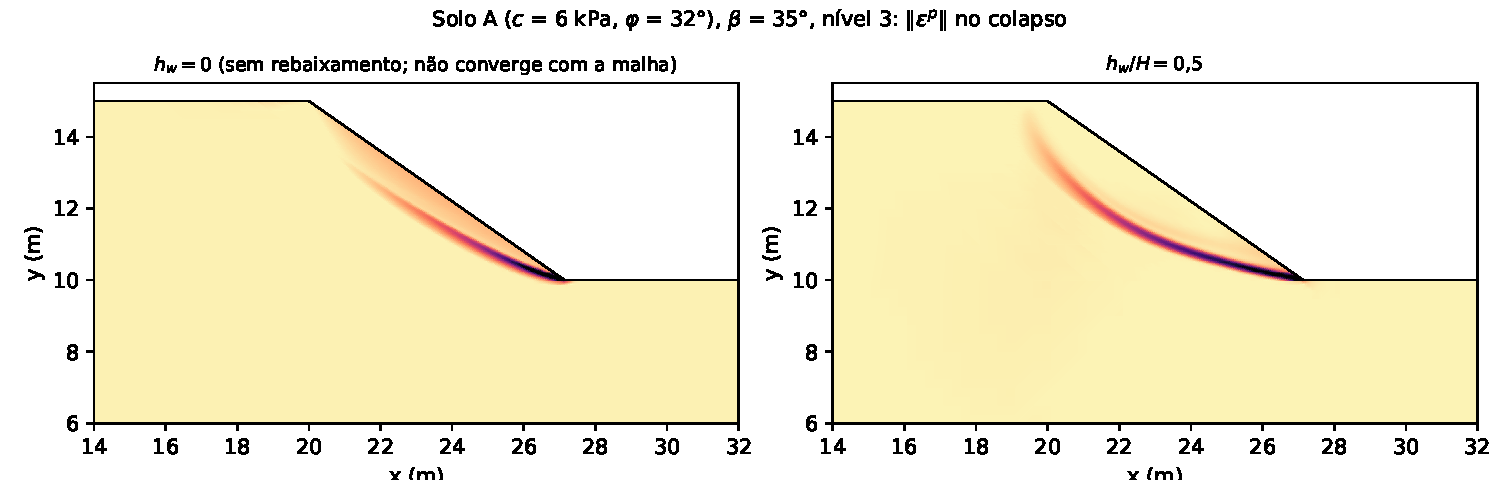
\includegraphics[width=\textwidth]{figuras/mecanismo_A35}\caption{Norma da deformação plástica no colapso, solo A ($c = 6$\,kPa, $\varphi = 32^\circ$), $\beta = 35^\circ$, nível 3: sem rebaixamento (esquerda; caso que não converge com a malha) e $h_w/H = 0{,}5$ (direita). Modelo com $H = 5$\,m e $\Hcrit = \Gam H$.}\label{fig:mec}\end{figure}
\subsection{Fig.~9 e Tabelas~5 e 6 do artigo: inclinação, anisotropia e rebaixamento}
\begin{figure}[H]\centering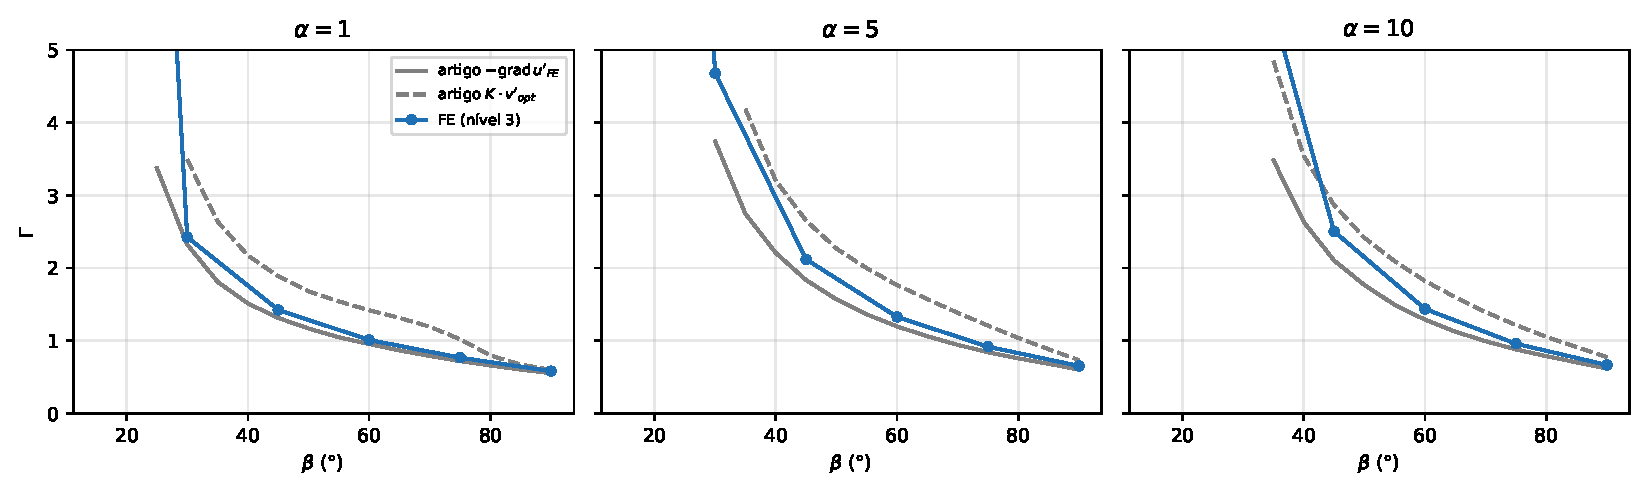
\includegraphics[width=\textwidth]{figuras/fig9_gamma_beta}\caption{$\Gam \times \beta$ para $\alpha = 1, 5, 10$ ($H = h_w = 5$\,m, $c = 10$\,kPa, $\varphi = 30^\circ$, $\gamma = 20$\,kN/m$^3$). Cinza: Fig.~9 do artigo (contínua ${\gradu}$, tracejada $\vopt$). Azul: FE, nível 3, crista 10\,m, pé 10\,m, base 5\,m.}\label{fig:f9}\end{figure}
\begin{table}[H]\centering\small\caption{Fig.~9 do artigo: FE (nível 3) contra a curva ${\gradu}$ do artigo (digitalizada da imagem, $\pm 0{,}01$; dif.\ calculada com os valores digitalizados sem arredondamento).}\label{tab:f9}\begin{tabular}{llrrrrr}\toprule $\alpha$ & & $\beta = 30^\circ$ & $\beta = 45^\circ$ & $\beta = 60^\circ$ & $\beta = 75^\circ$ & $\beta = 90^\circ$\\\midrule
1 & FE & 2{,}427 & 1{,}425 & 1{,}012 & 0{,}768 & 0{,}583\\
 & artigo & 2{,}33 & 1{,}31 & 0{,}96 & 0{,}72 & 0{,}55\\
 & dif. & $+$4{,}3\,\% & $+$8{,}4\,\% & $+$5{,}8\,\% & $+$6{,}6\,\% & $+$5{,}1\,\%\\
\addlinespace
5 & FE & 4{,}681 & 2{,}120 & 1{,}328 & 0{,}918 & 0{,}654\\
 & artigo & 3{,}75 & 1{,}83 & 1{,}20 & 0{,}84 & 0{,}60\\
 & dif. & $+$25{,}0\,\% & $+$15{,}5\,\% & $+$11{,}0\,\% & $+$9{,}0\,\% & $+$8{,}5\,\%\\
\addlinespace
10 & FE & 7{,}027 & 2{,}506 & 1{,}438 & 0{,}959 & 0{,}667\\
 & artigo & $> 5$ & 2{,}10 & 1{,}29 & 0{,}88 & 0{,}62\\
 & dif. & --- & $+$19{,}0\,\% & $+$11{,}5\,\% & $+$8{,}9\,\% & $+$7{,}9\,\%\\
\addlinespace
\bottomrule\end{tabular}\end{table}
Para $\alpha = 1$ o FE fica 4 a 8\,\% acima da curva ${\gradu}$, o mesmo resíduo do caso de referência; para $\alpha = 5$ e 10, 8 a 25\,\% acima. Na Tabela~\ref{tab:dom} ($\beta = 45^\circ$, $\alpha = 3$ e 5) o domínio grande reduz a diferença ao patamar de $\alpha = 1$; para $\alpha = 10$ e outros $\beta$ o efeito do domínio não foi verificado.
\begin{table}[H]\centering\small\caption{Coluna determinística das Tabelas~5 e 6 do artigo (domínio 10/10/5\,m).}\label{tab:t56}\begin{tabular}{lrrrr}\toprule caso & FE nível 2 (malha do MC) & FE nível 3 & artigo & dif. (nível 3)\\\midrule
$\alpha = 1$ & 1{,}453 & 1{,}425 & 1{,}336 & $+$6{,}6\,\%\\
$\alpha = 2$ & 1{,}703 & 1{,}665 & 1{,}533 & $+$8{,}6\,\%\\
$\alpha = 3$ & 1{,}886 & 1{,}847 & 1{,}674 & $+$10{,}3\,\%\\
$\alpha = 4$ & 2{,}031 & 2{,}005 & 1{,}783 & $+$12{,}4\,\%\\
$\alpha = 5$ & 2{,}156 & 2{,}120 & 1{,}872 & $+$13{,}3\,\%\\
$h_w/H = 0{,}5$ & 1{,}768 & 1{,}751 & 1{,}671 & $+$4{,}8\,\%\\
$h_w/H = 0{,}6$ & 1{,}586 & 1{,}578 & 1{,}494 & $+$5{,}6\,\%\\
$h_w/H = 0{,}7$ & 1{,}478 & 1{,}461 & 1{,}383 & $+$5{,}6\,\%\\
$h_w/H = 0{,}8$ & 1{,}423 & 1{,}402 & 1{,}322 & $+$6{,}0\,\%\\
$h_w/H = 0{,}9$ & 1{,}416 & 1{,}390 & 1{,}307 & $+$6{,}3\,\%\\
\bottomrule\end{tabular}\end{table}
\section{Monte Carlo}
Nas tabelas, $\mu$, $\sigma$ e CoV são de $\Gam$; Pf com o intervalo de confiança de 95\,\%; as colunas com~$^*$ são as reescaladas pelo $\Gam$ determinístico (seção~2.2); as três últimas colunas, em vermelho, são os valores do artigo.
\begin{table}[H]\centering\footnotesize\setlength{\tabcolsep}{3.2pt}\caption{Monte Carlo, casos da Tabela 3 do artigo: coeficientes de variação}\label{tab:mc3}
\begin{tabular}{lrrrrlrrr>{\color{art}}r>{\color{art}}r>{\color{art}}r}\toprule & \multicolumn{5}{c}{FE} & \multicolumn{3}{c}{FE reescalado} & \multicolumn{3}{c}{\color{art}artigo}\\\cmidrule(lr){2-6}\cmidrule(lr){7-9}\cmidrule(l){10-12}caso & $N$ & $\mu$ & $\sigma$ & CoV\,\% & Pf\,\% (IC 95\,\%) & $\mu^*$ & $\sigma^*$ & Pf$^*$\,\% & $\mu$ & $\sigma$ & Pf\,\%\\\midrule
referência & 500 & 1{,}461 & 0{,}383 & 26{,}2 & 8{,}60 (6{,}4--11{,}4) & 1{,}343 & 0{,}352 & 15{,}20 & 1{,}353 & 0{,}318 & 11{,}50\\
$\mathrm{CoV}(k_v) = 0$ & 500 & 1{,}420 & 0{,}335 & 23{,}6 & 8{,}00 (5{,}9--10{,}7) & 1{,}306 & 0{,}309 & 16{,}40 & 1{,}329 & 0{,}288 & 11{,}21\\
$\mathrm{CoV}(k_v) = 75\,\%$ & 500 & 1{,}480 & 0{,}406 & 27{,}4 & 8{,}00 (5{,}9--10{,}7) & 1{,}361 & 0{,}373 & 15{,}40 & 1{,}375 & 0{,}341 & 11{,}41\\
$\mathrm{CoV}(k_v) = 90\,\%$ & 496 & 1{,}502 & 0{,}434 & 28{,}9 & 8{,}27 (6{,}2--11{,}0) & 1{,}382 & 0{,}400 & 15{,}32 & 1{,}378 & 0{,}354 & 11{,}63\\
$\mathrm{CoV}(k_v) = 100\,\%$ & 490 & 1{,}516 & 0{,}455 & 30{,}0 & 8{,}57 (6{,}4--11{,}4) & 1{,}394 & 0{,}418 & 15{,}31 & 1{,}391 & 0{,}360 & 11{,}44\\
$\mathrm{CoV}(c) = 10\,\%$ & 476 & 1{,}493 & 0{,}238 & 15{,}9 & 0{,}00 (0{,}0--0{,}8) & 1{,}373 & 0{,}219 & 1{,}26 & 1{,}367 & 0{,}180 & 0{,}45\\
$\mathrm{CoV}(c) = 50\,\%$ & 473 & 1{,}419 & 0{,}539 & 38{,}0 & 23{,}26 (19{,}7--27{,}3) & 1{,}304 & 0{,}495 & 28{,}33 & 1{,}324 & 0{,}472 & 25{,}78\\
$\mathrm{CoV}(c) = 70\,\%$ & 471 & 1{,}354 & 0{,}664 & 49{,}0 & 33{,}97 (29{,}8--38{,}4) & 1{,}245 & 0{,}610 & 40{,}55 & 1{,}296 & 0{,}620 & 36{,}34\\
$\mathrm{CoV}(\varphi) = 5\,\%$ & 454 & 1{,}465 & 0{,}358 & 24{,}5 & 7{,}27 (5{,}2--10{,}0) & 1{,}347 & 0{,}329 & 14{,}76 & 1{,}351 & 0{,}300 & 10{,}20\\
$\mathrm{CoV}(\varphi) = 15\,\%$ & 450 & 1{,}479 & 0{,}442 & 29{,}9 & 11{,}33 (8{,}7--14{,}6) & 1{,}360 & 0{,}407 & 17{,}11 & 1{,}357 & 0{,}346 & 12{,}71\\
$\mathrm{CoV}(\varphi) = 20\,\%$ & 450 & 1{,}486 & 0{,}520 & 35{,}0 & 14{,}00 (11{,}1--17{,}5) & 1{,}366 & 0{,}478 & 19{,}78 & 1{,}361 & 0{,}384 & 15{,}18\\
\bottomrule\end{tabular}
\end{table}
\begin{table}[H]\centering\footnotesize\setlength{\tabcolsep}{3.2pt}\caption{Monte Carlo, casos da Tabela 4 do artigo: distâncias de autocorrelação $(L_x, L_y) = s\,(20\ \mathrm{m}, 2\ \mathrm{m})$}\label{tab:mc4}
\begin{tabular}{lrrrrlrrr>{\color{art}}r>{\color{art}}r>{\color{art}}r}\toprule & \multicolumn{5}{c}{FE} & \multicolumn{3}{c}{FE reescalado} & \multicolumn{3}{c}{\color{art}artigo}\\\cmidrule(lr){2-6}\cmidrule(lr){7-9}\cmidrule(l){10-12}caso & $N$ & $\mu$ & $\sigma$ & CoV\,\% & Pf\,\% (IC 95\,\%) & $\mu^*$ & $\sigma^*$ & Pf$^*$\,\% & $\mu$ & $\sigma$ & Pf\,\%\\\midrule
referência & 500 & 1{,}461 & 0{,}383 & 26{,}2 & 8{,}60 (6{,}4--11{,}4) & 1{,}343 & 0{,}352 & 15{,}20 & 1{,}353 & 0{,}318 & 11{,}50\\
$s = 1{,}5$ & 450 & 1{,}475 & 0{,}447 & 30{,}3 & 10{,}22 (7{,}8--13{,}4) & 1{,}356 & 0{,}411 & 17{,}78 & 1{,}356 & 0{,}352 & 13{,}94\\
$s = 2$ & 450 & 1{,}474 & 0{,}444 & 30{,}1 & 12{,}22 (9{,}5--15{,}6) & 1{,}356 & 0{,}408 & 18{,}22 & 1{,}361 & 0{,}372 & 14{,}99\\
$s = 5$ & 450 & 1{,}461 & 0{,}468 & 32{,}0 & 13{,}33 (10{,}5--16{,}8) & 1{,}344 & 0{,}430 & 23{,}56 & 1{,}350 & 0{,}404 & 18{,}93\\
$s = 10$ & 450 & 1{,}465 & 0{,}480 & 32{,}8 & 14{,}44 (11{,}5--18{,}0) & 1{,}347 & 0{,}441 & 22{,}67 & 1{,}348 & 0{,}419 & 19{,}85\\
$s = 20$ & 450 & 1{,}456 & 0{,}478 & 32{,}8 & 14{,}44 (11{,}5--18{,}0) & 1{,}339 & 0{,}439 & 23{,}11 & 1{,}355 & 0{,}430 & 20{,}23\\
$s = 400$ & 450 & 1{,}453 & 0{,}490 & 33{,}8 & 14{,}67 (11{,}7--18{,}2) & 1{,}336 & 0{,}451 & 24{,}22 & 1{,}348 & 0{,}432 & 21{,}93\\
\bottomrule\end{tabular}
\end{table}
\begin{table}[H]\centering\footnotesize\setlength{\tabcolsep}{3.2pt}\caption{Monte Carlo, casos da Tabela 5 do artigo: anisotropia $\alpha = k_h/k_v$}\label{tab:mc5}
\begin{tabular}{lrrrrlrrr>{\color{art}}r>{\color{art}}r>{\color{art}}r}\toprule & \multicolumn{5}{c}{FE} & \multicolumn{3}{c}{FE reescalado} & \multicolumn{3}{c}{\color{art}artigo}\\\cmidrule(lr){2-6}\cmidrule(lr){7-9}\cmidrule(l){10-12}caso & $N$ & $\mu$ & $\sigma$ & CoV\,\% & Pf\,\% (IC 95\,\%) & $\mu^*$ & $\sigma^*$ & Pf$^*$\,\% & $\mu$ & $\sigma$ & Pf\,\%\\\midrule
referência & 500 & 1{,}461 & 0{,}383 & 26{,}2 & 8{,}60 (6{,}4--11{,}4) & 1{,}343 & 0{,}352 & 15{,}20 & 1{,}353 & 0{,}318 & 11{,}50\\
$\alpha = 2$ & 450 & 1{,}733 & 0{,}494 & 28{,}5 & 3{,}11 (1{,}9--5{,}2) & 1{,}560 & 0{,}444 & 6{,}44 & 1{,}562 & 0{,}390 & 3{,}90\\
$\alpha = 3$ & 450 & 1{,}928 & 0{,}574 & 29{,}7 & 1{,}11 (0{,}5--2{,}6) & 1{,}711 & 0{,}509 & 4{,}22 & 1{,}704 & 0{,}432 & 1{,}83\\
$\alpha = 4$ & 450 & 2{,}080 & 0{,}635 & 30{,}5 & 0{,}67 (0{,}2--1{,}9) & 1{,}826 & 0{,}558 & 2{,}44 & 1{,}821 & 0{,}474 & 1{,}00\\
$\alpha = 5$ & 450 & 2{,}205 & 0{,}688 & 31{,}2 & 0{,}22 (0{,}0--1{,}2) & 1{,}914 & 0{,}597 & 1{,}56 & 1{,}910 & 0{,}504 & 0{,}63\\
\bottomrule\end{tabular}
\end{table}
\begin{table}[H]\centering\footnotesize\setlength{\tabcolsep}{3.2pt}\caption{Monte Carlo, casos da Tabela 6 do artigo: rebaixamento $h_w/H$}\label{tab:mc6}
\begin{tabular}{lrrrrlrrr>{\color{art}}r>{\color{art}}r>{\color{art}}r}\toprule & \multicolumn{5}{c}{FE} & \multicolumn{3}{c}{FE reescalado} & \multicolumn{3}{c}{\color{art}artigo}\\\cmidrule(lr){2-6}\cmidrule(lr){7-9}\cmidrule(l){10-12}caso & $N$ & $\mu$ & $\sigma$ & CoV\,\% & Pf\,\% (IC 95\,\%) & $\mu^*$ & $\sigma^*$ & Pf$^*$\,\% & $\mu$ & $\sigma$ & Pf\,\%\\\midrule
$h_w/H = 0{,}5$ & 450 & 1{,}779 & 0{,}442 & 24{,}9 & 2{,}00 (1{,}1--3{,}8) & 1{,}682 & 0{,}418 & 2{,}89 & 1{,}670 & 0{,}378 & 1{,}38\\
$h_w/H = 0{,}6$ & 450 & 1{,}608 & 0{,}403 & 25{,}1 & 4{,}44 (2{,}9--6{,}8) & 1{,}514 & 0{,}379 & 6{,}44 & 1{,}502 & 0{,}345 & 4{,}20\\
$h_w/H = 0{,}7$ & 450 & 1{,}501 & 0{,}380 & 25{,}3 & 6{,}89 (4{,}9--9{,}6) & 1{,}405 & 0{,}356 & 10{,}44 & 1{,}393 & 0{,}314 & 8{,}54\\
$h_w/H = 0{,}8$ & 450 & 1{,}444 & 0{,}371 & 25{,}7 & 9{,}33 (7{,}0--12{,}4) & 1{,}342 & 0{,}345 & 16{,}22 & 1{,}338 & 0{,}309 & 11{,}99\\
$h_w/H = 0{,}9$ & 450 & 1{,}435 & 0{,}373 & 26{,}0 & 10{,}22 (7{,}8--13{,}4) & 1{,}325 & 0{,}344 & 17{,}78 & 1{,}325 & 0{,}306 & 12{,}58\\
referência & 500 & 1{,}461 & 0{,}383 & 26{,}2 & 8{,}60 (6{,}4--11{,}4) & 1{,}343 & 0{,}352 & 15{,}20 & 1{,}353 & 0{,}318 & 11{,}50\\
\bottomrule\end{tabular}
\end{table}
\begin{table}[H]\centering\footnotesize\setlength{\tabcolsep}{3.2pt}\caption{Monte Carlo, exemplos de Cho (2010) da seção 5.3 do artigo, sem percolação}\label{tab:mccho}
\begin{tabular}{lrrrrlrrr>{\color{art}}r>{\color{art}}r>{\color{art}}r}\toprule & \multicolumn{5}{c}{FE} & \multicolumn{3}{c}{FE reescalado} & \multicolumn{3}{c}{\color{art}artigo}\\\cmidrule(lr){2-6}\cmidrule(lr){7-9}\cmidrule(l){10-12}caso & $N$ & $\mu$ & $\sigma$ & CoV\,\% & Pf\,\% (IC 95\,\%) & $\mu^*$ & $\sigma^*$ & Pf$^*$\,\% & $\mu$ & $\sigma$ & Pf\,\%\\\midrule
Cho, coesivo & 390 & 1{,}232 & 0{,}199 & 16{,}2 & 10{,}77 (8{,}1--14{,}2) & 1{,}258 & 0{,}203 & 8{,}97 & 1{,}279$^\dagger$ & 0{,}201 & 6{,}50\\
Cho, $c$-$\varphi$ & 450 & 1{,}871 & 1{,}129 & 60{,}3 & 7{,}56 (5{,}5--10{,}4) & 1{,}838 & 1{,}109 & 8{,}22 & 1{,}866$^\dagger$ & 0{,}82--0{,}94 & 5{,}50\\
\bottomrule\end{tabular}
\\[2pt]\parbox{\linewidth}{\footnotesize $^\dagger$ $\mu$ e $\sigma$ do artigo calculados das curvas das Figs.~17, 21 e 22 do artigo (não tabelados); no $c$-$\varphi$ a densidade da Fig.~21 é cortada na cauda e a CDF da Fig.~22 dá $\mu = 1{,}90$ e $\sigma = 0{,}94$. Pf de Cho (2010): 7,9\,\% (coesivo) e 6,37\,\% ($c$-$\varphi$).}
\end{table}
\subsection{Exemplos de Cho}
No talude coesivo a distribuição de $\Gam$ do FE é quase a do artigo ($\mu = 1{,}232$ e $\sigma = 0{,}199$ contra 1{,}279 e 0{,}201); a média um pouco menor acompanha o $\Gam$ determinístico do FE na malha do Monte Carlo (1{,}325 contra 1,354) e leva a um Pf maior (10{,}8\,\%, ou 9{,}0\,\% reescalado, contra 6,5\,\% no artigo e 7,9\,\% em Cho). No talude $c$-$\varphi$ os quantis do FE e do artigo (CDF da Fig.~22) são próximos: 5\,\%: 0{,}95 e 0{,}99, 25\,\%: 1{,}29 e 1{,}32, 75\,\%: 2{,}19 e 2{,}18, 95\,\%: 3{,}40 e 3{,}58; mediana 1{,}67 e 1{,}67. O desvio padrão maior do FE (1{,}129) vem da cauda superior: uma amostra tem $\Gam = 17{,}4$ e, sem ela, $\sigma = 0{,}859$.
\begin{figure}[H]\centering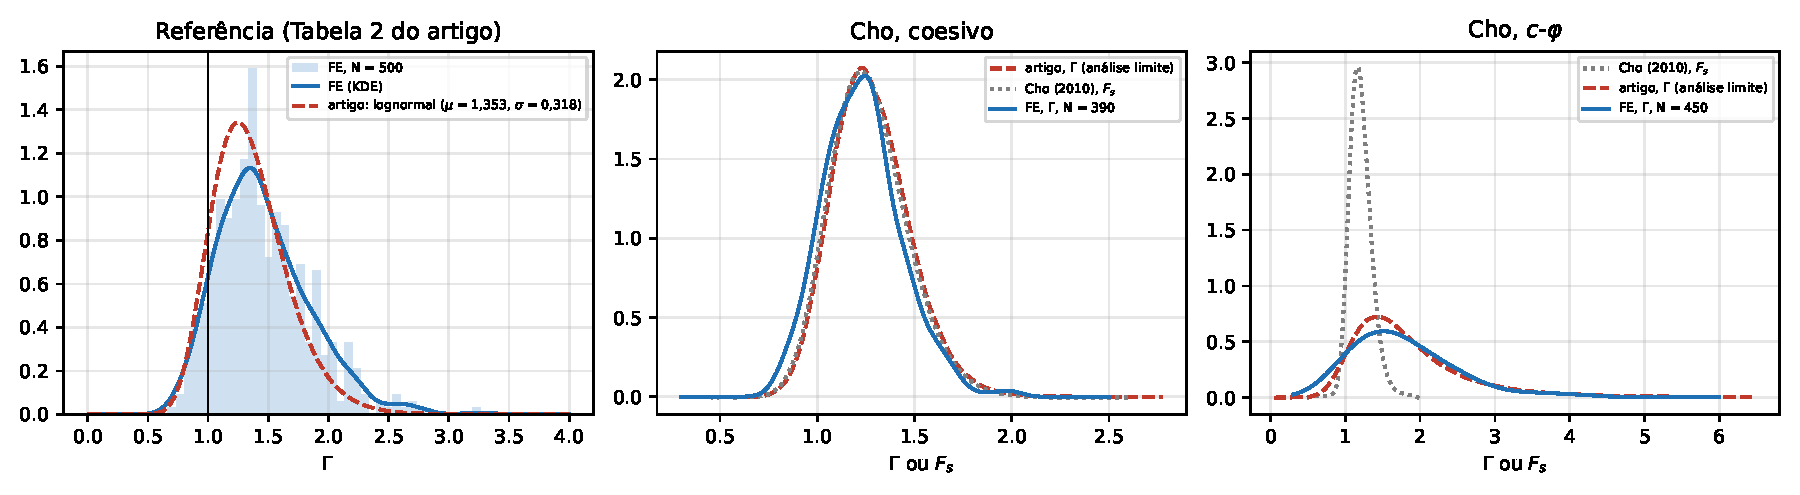
\includegraphics[width=\textwidth]{figuras/densidades}\caption{Densidade de $\Gam$: referência (lognormal do artigo, $\mu = 1{,}353$, $\sigma = 0{,}318$) e exemplos de Cho (curvas do artigo extraídas das Figs.~17 e 21, com a densidade de $F_s$ de Cho).}\label{fig:dens}\end{figure}
\subsection{Casos com percolação (Tabelas~3 a 6 do artigo)}
\begin{figure}[H]\centering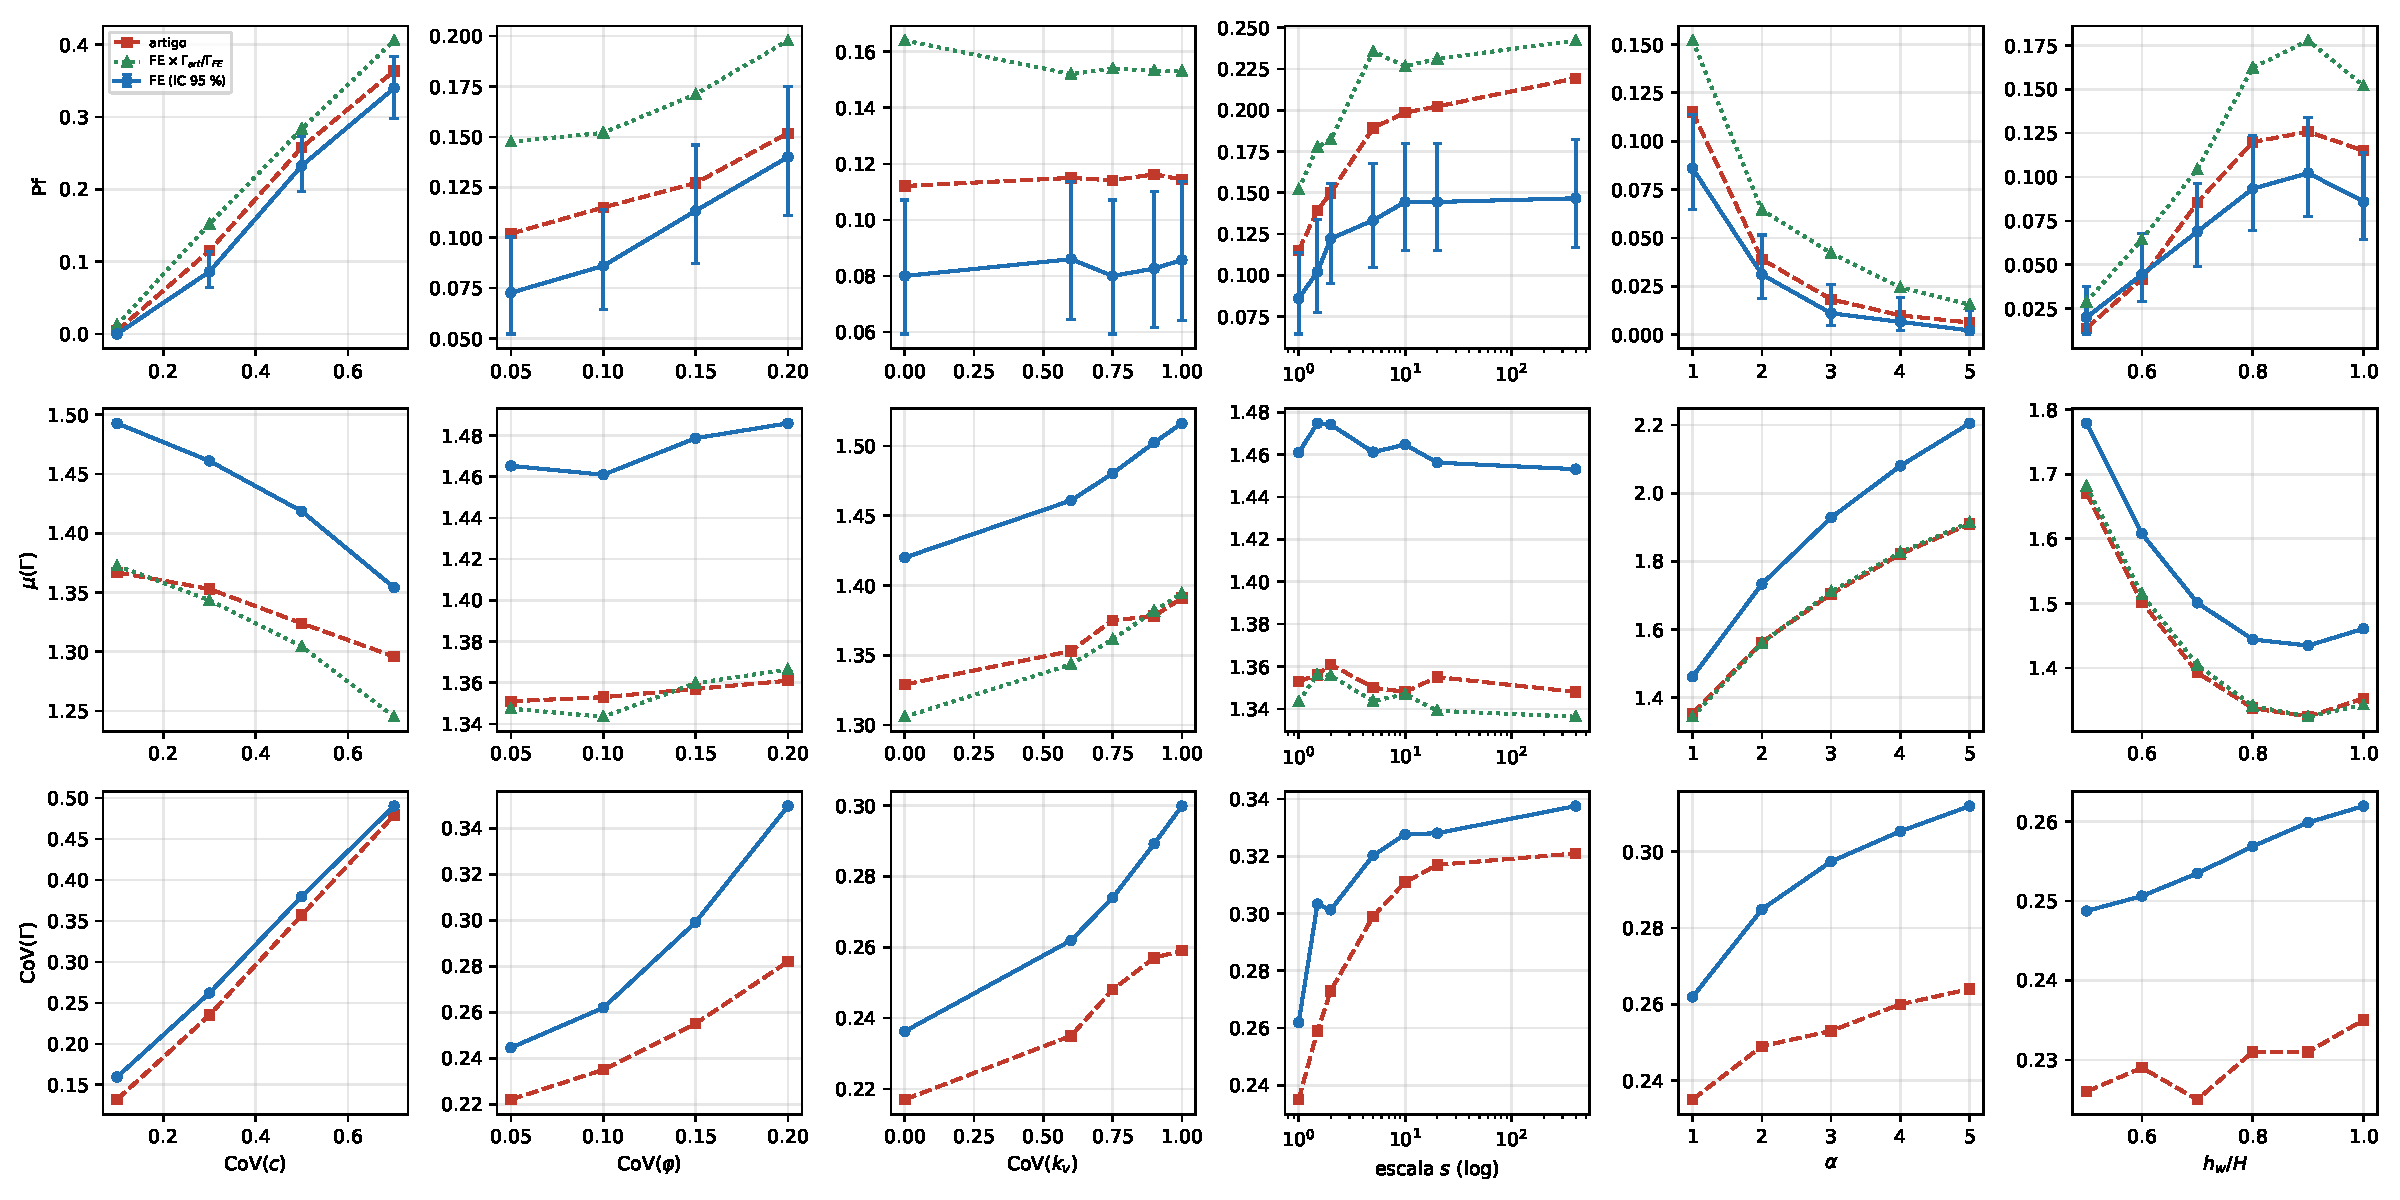
\includegraphics[width=\textwidth]{figuras/tendencias}\caption{Tendências das Tabelas~3 a 6 do artigo (Tabelas~\ref{tab:mc3} a \ref{tab:mc6}): Pf, $\mu(\Gam)$ e CoV$(\Gam)$. Vermelho: artigo; azul: FE (barras: IC de 95\,\% de Pf); verde: FE reescalado. Eixo de $s$ em escala logarítmica.}\label{fig:tend}\end{figure}
Nos 26 casos com percolação: (i) a média do FE é 8{,}8\,\% maior que a do artigo, o mesmo viés do problema médio na malha do Monte Carlo (Tabela~\ref{tab:t56}); reescalada, coincide com a do artigo (diferença média $-$0{,}3\,\%); (ii) o desvio padrão reescalado é 12\,\% maior em média. Hipóteses para (ii), não testadas aqui: o FE forma mecanismos que seguem as zonas fracas, enquanto a família de superfícies log-espirais média a resistência ao longo de curvas suaves (efeito conhecido do RFEM); o artigo trunca a KL sem compensar a variância perdida; e usa em cada arco o $\varphi$ máximo do subdomínio, o que suaviza os valores baixos. (iii) Com isso o Pf do artigo fica entre o Pf do FE e o reescalado em 24 dos 26 casos (exceções: $h_w/H = 0{,}5$ e $h_w/H = 0{,}6$, com Pf do FE já maior que o do artigo). As tendências principais se repetem: Pf cresce muito com CoV$(c)$, pouco com CoV$(\varphi)$ e quase nada com CoV$(k_v)$; cresce com a escala $s$ das distâncias de autocorrelação; cai com $\alpha$; e o mínimo de estabilidade ocorre perto de $h_w/H = 0{,}8$--$0{,}9$; $\sigma$ e CoV crescem com $s$. Variações pequenas ($\mu$ com CoV$(\varphi)$ e com $s$, oscilações de $\sigma$ entre valores vizinhos de $s$) ficam dentro do ruído amostral.
Nos casos com Pf pequeno ainda há poucas falhas (por exemplo, $\alpha = 5$: 1 em 450), e o Pf deles só fica bem determinado com muito mais amostras (seção~\ref{sec:prev}).
\begin{figure}[H]\centering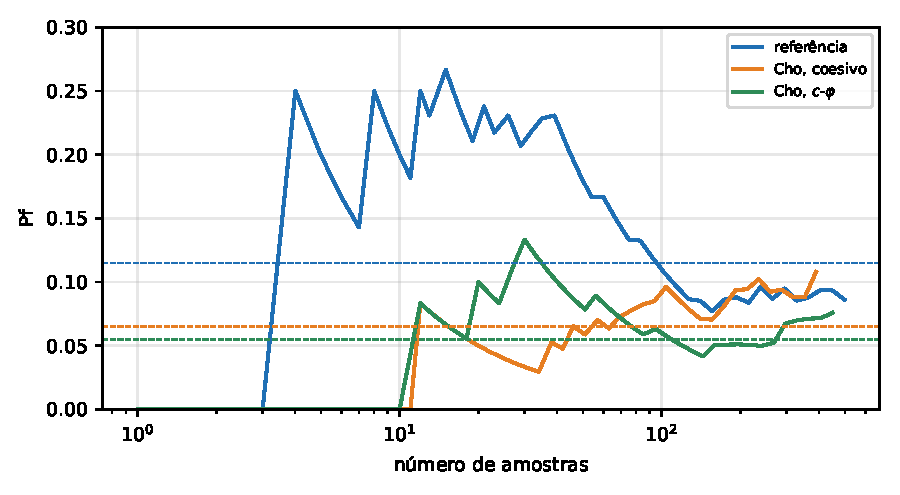
\includegraphics[width=0.62\textwidth]{figuras/convergencia_pf}\caption{Convergência de Pf com o número de amostras (tracejadas: valores do artigo).}\label{fig:conv}\end{figure}
\subsection{Sensibilidade (seção 6.1 e Fig.~26 do artigo)}
\begin{table}[H]\centering\small\caption{Correlação parcial de Spearman de 2ª ordem entre $\Gam$ e cada variável (caso de referência, $N = 500$).}\begin{tabular}{lrrr}\toprule variável & FE, médias no mecanismo & FE, médias no domínio & artigo\\\midrule
$c$ & 0{,}878 & 0{,}818 & 0,879\\
$\varphi$ & 0{,}550 & 0{,}481 & 0,508\\
$k_v$ & $-$0{,}213 & 0{,}071 & $-$0,036\\
\bottomrule\end{tabular}\end{table}
Médias no mecanismo: $c$ e $\varphi$ médios na banda de cisalhamento ($\|\Delta\varepsilon^p\| \ge 10\,\%$ do máximo no colapso, ponderados por $\|\Delta\varepsilon^p\|$) e $k_v$ médio na massa que se move ($\|\Delta u\| \ge 30\,\%$ do máximo), análogas às médias ao longo da superfície de ruptura e no volume deslizante usadas no artigo (Hu et al.).
\subsection{Modos de ruptura (Figs.~16 e 20 do artigo)}
\begin{table}[H]\centering\small\caption{Modos de ruptura: banda $\|\Delta\varepsilon^p\| \ge 20\,\%$ do máximo no colapso; abaixo do pé se ela desce mais de $0{,}1H$ abaixo do nível do pé, pelo pé se passa a menos de $0{,}1H$ do pé.}\begin{tabular}{lrrrrl}\toprule exemplo & $N$ & acima & pelo pé & abaixo & artigo (acima/pelo/abaixo)\\\midrule
Cho, coesivo & 390 & 0{,}0\,\% & 0{,}0\,\% & 100{,}0\,\% & 0,55 / 6,76 / 92,68\,\%\\
Cho, $c$-$\varphi$ & 450 & 5{,}1\,\% & 94{,}9\,\% & 0{,}0\,\% & 19,20 / 80,80 / 0\,\%\\
referência & 500 & 0{,}2\,\% & 95{,}0\,\% & 4{,}8\,\% & ---\\
\bottomrule\end{tabular}\end{table}
\section{Observações sobre o artigo}\label{sec:obs}
\begin{enumerate}
\item \textbf{Fig.~8 com os solos trocados.} Sem rebaixamento ($h_w/H = 0$), a solução log-espiral de Chen (1975)
com $\gamma' = 18 - 9{,}81$ dá, para $c = 6$\,kPa e $\varphi = 32^\circ$ (``London clay'' na Tabela~1 do artigo),
$\Hcrit = 13{,}00$\,m ($\beta = 60^\circ$) e $229{,}1$\,m ($\beta = 35^\circ$), que são as curvas do painel ``Israeli
Clay'' (12,98\,m e 229,3\,m, este fora da escala impressa, lido do vetor do PDF); para $c = 11{,}7$\,kPa e
$\varphi = 24{,}7^\circ$ dá 17,97\,m ($\beta = 60^\circ$) e 156,7\,m ($\beta = 30^\circ$), as do painel ``London
Clay'' (17,95 e 156,6\,m). Para $\varphi = 32^\circ$, $\beta = 35^\circ$ o FE não converge com a malha
(seção~\ref{sec:f8}); nas outras três curvas ele dá os mesmos valores (13{,}19\,m, 18{,}07\,m, 153{,}21\,m, diferença de 0,7 a
2,1\,\%, nível 3).
\item \textbf{$\gamma_w$ não informado.} Os valores da Fig.~8 do artigo sem rebaixamento só são reproduzidos com
$\gamma_w = 9{,}81$\,kN/m$^3$.
\item \textbf{Altura do exemplo $c$-$\varphi$ de Cho.} O texto da seção~5.3.2 e o rótulo da cota da Fig.~19 do
artigo dão $H = 5$\,m (o desenho, em escala, tem $H = 10$\,m e $30 \times 15$\,m), mas $\Gam = 1{,}777$ e
$F_s = 1{,}203/1{,}204$ correspondem a $H = 10$\,m: Chen dá $\Gam = 1{,}7770$ e $F_s = 1{,}203$ com $H = 10$\,m, e
3,554 e 1,60 com $H = 5$\,m.
\item \textbf{Seção 6.1.} O texto fala em correlação ``perfeita'' de $\Gam$ com a coesão, mas a barra da Fig.~26 do
artigo vale 0,88.
\item \textbf{Forças de percolação do caso de referência.} Mesmo usando a mesma aproximação (${\gradu}$), o FE
convergido fica acima do $\Gam = 1{,}336$ do artigo (seção~\ref{sec:conv}), o que aponta para uma diferença na solução
hidráulica (malha e domínio do FE hidráulico do artigo não são informados).
\item \textbf{Limite superior com $\varphi$ próximo de $\beta$.} No solo A com $\beta = 35^\circ$ o FE fica
16 a 26\,\% abaixo do limite superior do artigo para $h_w/H \ge 0{,}2$ e continua diminuindo com o
refinamento, com um mecanismo raso junto à face (seção~\ref{sec:f8}).
\end{enumerate}

\section{Previsão de tempo}\label{sec:prev}
Tempo por amostra medido na máquina do autor com 8 processos simultâneos: 3{,}4 a 4{,}2\,s nos casos com percolação, 2{,}4\,s no Cho $c$-$\varphi$ e 36{,}6\,s no Cho coesivo (malha de 18 mil equações). A Tabela~\ref{tab:prev} dá o que falta a partir das 12.850 amostras já calculadas.
\begin{table}[H]\centering\small\caption{Tempo que falta, a partir das amostras atuais. A coluna de 16 processos supõe 16 núcleos físicos e o mesmo tempo por amostra.}\label{tab:prev}\begin{tabular}{lrrrr}\toprule meta por caso & amostras no total & CPU (h) & 8 processos & 16 processos\\\midrule
$N = 1000$ & 28.000 & 22 & 2{,}7\,h & 1{,}4\,h\\
$N = 2000$ & 56.000 & 61 & 7{,}6\,h & 3{,}8\,h\\
CoV(Pf) $< 5\,\%$ com o Pf do FE$^d$ & 478.250 & 531 & 66\,h (2{,}8 d) & 33{,}2\,h\\
$S$ do artigo (10 mil a 100 mil) & 630.000 & 1555 & 194\,h (8{,}1 d) & 97\,h (4{,}1 d)\\
\bottomrule\end{tabular}\\[2pt]\parbox{\linewidth}{\footnotesize $^d$ fórmula aplicada ao Pf atual de cada caso (no mínimo 1000, em blocos de 50); muito incerta onde há poucas falhas: $\alpha = 5$ tem 1 falha em 450 amostras, e o alvo dele vai de cerca de 30 mil a 1 milhão de amostras no intervalo de confiança de Pf. Casos ainda sem falhas usam o $S$ do artigo: $\mathrm{CoV}(c) = 10\,\%$, 90.000 amostras (cerca de 100\,h de CPU).}\end{table}
No alvo do artigo o Cho coesivo responde por 1014 das 1555\,h de CPU que faltam. Com $h = 2$\,m nesse caso (cerca de 7 mil equações) o custo por amostra cai para cerca de um quinto (medição no container de desenvolvimento, 4 amostras simultâneas: 6,4\,s com $h = 2$\,m contra 29,7\,s com $h = 1$\,m), com $\Gam$ cerca de 1\,\% maior. Na ferramenta, \texttt{-{}-alvo cov5} leva primeiro cada caso a 1000 amostras (\texttt{-{}-min}) e reavalia o alvo cada vez que a fila é gerada de novo.
\section{Reprodução}
{\sloppy Branch \texttt{claude/great-clarke-xist30} do neopz-master; dados, logs, figuras e este relatório em
\texttt{Projects2/SlopeSeepageRandom/resultados/artigo2025/} (\texttt{campanha/}: amostras juntadas;
\texttt{det/}: logs determinísticos; \texttt{ref/}: dados extraídos do artigo; \texttt{relatorio\_tex/}: este
documento).\par}
\par\noindent\begin{minipage}{\textwidth}\footnotesize
\begin{verbatim}
sudo apt install cmake g++ make liblapack-dev libblas-dev liblapacke-dev \
     python3-numpy python3-scipy python3-matplotlib texlive-latex-extra texlive-lang-portuguese
# Monte Carlo: compila, gera a fila (blocos de 50 amostras, casos intercalados) e roda
bash Projects2/SlopeSeepageRandom/scripts/rodar_campanha.sh 1000   # [N|cov5|artigo] [proc.] [dir]
S=$PWD/Projects2/SlopeSeepageRandom/scripts
A=$PWD/Projects2/SlopeSeepageRandom/resultados/artigo2025
PROCESSOS=8 python3 $S/campanha_artigo.py status ~/campanha_artigo
# análise (campanha: ~/campanha_artigo ou $A/campanha) e relatórios
python3 $S/analise_artigo.py ~/campanha_artigo $A/det $A/ref saida
python3 $S/relatorio_tex.py saida relatorio_tex
cd relatorio_tex && for i in 1 2 3; do pdflatex relatorio.tex; done
\end{verbatim}
\end{minipage}
\end{document}
